\chapter{The Cost of ``This Has Nothing to Do with Me''}

One of the most expensive mistakes in life does not feel like a mistake when it happens.

It feels reasonable.

A person hears an idea, understands the words, even nods sincerely. The idea may be correct. It may be important. It may be exactly the idea that could change his path. Yet somewhere inside, a quiet sentence appears:

\begin{quote}
Yes, but this has nothing to do with me.
\end{quote}

That sentence is dangerous because it does not sound lazy. It sounds modest. It sounds practical. It sounds like self-knowledge.

``I am not that kind of person.''

``My situation is different.''

``I cannot do what he does.''

``I should just focus on what I can already do.''

Sometimes those sentences are true. More often, they are a polite mask for avoidance. The mind wants to stay in the familiar world, so it classifies the new idea as unrelated. Once the idea is classified that way, it cannot work. Not because the idea is wrong, but because it has been denied entry.

\section*{A Missed Afternoon}

In the summer of 2007, near the end of my time teaching at New Oriental, a young woman handed me a business card after class.

``A friend of mine would like to meet you. Would that be possible?''

I said yes almost casually. I was leaving soon, or at least I thought I was leaving soon. In fact, my departure from New Oriental dragged on for several semesters. Each time I said it would be my last course, the department needed another teacher, and I agreed to teach again. The final leaving was not as clean as the story sounds in memory.

A few days later I found the card and called the person on it. Let us call him Zhuang Yi. His title said that he was a founding partner of a well-known venture capital firm.

At that time, this meant almost nothing to me. I had heard of venture capital, perhaps, but I did not really know what it was. I had no real contact with that world. Like many teachers in a comfortable and closed environment, I knew my own classroom, my own students, my own income, and my own small circle. The outside world was moving, but I was not paying enough attention.

Comfort often produces this blindness. Inside the enclosure, everything feels fine. Only after being pushed outside does a person realize how little preparation he made.

Zhuang Yi had been invited to Stanford for an MBA. The school had apparently made the process easy for him, but he still felt he should take the required tests properly. His schedule was chaotic, so his assistant attended several TOEFL and GMAT classes, sampled different teachers, and finally brought him my card.

We met. I explained the test systems quickly, went through the important points, and then met him once or twice a week for details. I slowly learned that he was a remarkable figure in the venture capital world. I also noticed his working style. He flew constantly, slept only a few hours on many days, completed assignments in airports, and still made time to review them carefully.

People who are ruthless with execution are easy to respect.

Before he left for San Francisco, he said, in effect, ``You have taught me a lot. Let me teach you once. I will explain entrepreneurship.''

He stood by a whiteboard for two and a half hours. He filled the board, erased it, filled it again, and kept going. It was about the length of one of my own full classes.

What did he say?

For years, I could not remember.

I remembered the scene. I remembered the whiteboard. I remembered that what he said must have been important. But the details were almost completely gone.

Two years passed. He returned from Stanford. My own life had not changed much. I was running an overseas education consulting business with a former colleague. It made money, but in hindsight it was not a startup in any meaningful sense. It was a business, and a small one. There was no real growth engine, no large ambition, no understanding of the long track.

In 2013 I began angel investing. In early 2014 I went to Silicon Valley. On the plane, the memory of that afternoon came back suddenly: Zhuang Yi standing in that room, writing on the whiteboard, explaining entrepreneurship to me.

The feeling was like waking from a bad dream.

I tried to recall the content. I could not. The more I tried, the clearer the truth became:

\begin{quote}
I had not really listened.
\end{quote}

I had heard the words. I had respected the person. I had probably nodded in the right places. But the ideas had not entered me.

\section*{Understanding Is Not Entry}

Many readers experience the same thing with books, essays, lectures, and conversations.

At the moment of reading, they feel clarity. The sentences are smooth. The argument seems right. The mind enjoys the recognition: ``Exactly. This is true.''

Then a month later, if they are asked what they actually absorbed, there is little left. A vague impression remains, but no usable method, no changed behavior, no new decision rule.

The pleasure of reading creates a false certificate of understanding.

The same happens in conversation. A person can sit across from someone wiser, more experienced, and more capable, and still fail to receive the useful part. The problem is not ears. The problem is classification.

At that time, I had probably classified Zhuang Yi's lesson as something like this:

\begin{quote}
This is correct, impressive, and profound, but it does not have much to do with me.
\end{quote}

I was not a venture capitalist. I was not a Silicon Valley founder. I was a teacher who had built a decent income and a small business. So my mind politely placed his ideas on a distant shelf.

That shelf is where many life-changing ideas go to die.

\section*{The Self-Fulfilling Distance}

The most damaging form of rejection is not disagreement. Disagreement can be useful. If you disagree seriously, you may still think, compare, test, and argue. The idea remains alive.

The deeper danger is distance.

``It has nothing to do with me'' kills the idea before it can be tested.

Some ideas will not help you even if you believe they are relevant. You may misunderstand them. You may apply them badly. The timing may be wrong. Your conditions may not yet support them.

But the reverse is certain:

\begin{quote}
If you decide that an idea has nothing to do with you, it will not work for you.
\end{quote}

This is why the sentence is a self-fulfilling prophecy. Once the mind declares distance, attention withdraws. Because attention withdraws, no action follows. Because no action follows, no feedback appears. Because no feedback appears, the idea never becomes part of life. Later the person says, ``See? It really had nothing to do with me.''

The conclusion was built into the first classification.

\begin{center}
\begin{adjustbox}{max width=\linewidth}
\begin{tikzpicture}[
  box/.style={draw, rounded corners=2pt, align=center, minimum width=2.65cm, minimum height=0.85cm},
  arrow/.style={->, thick}
]
\node[box] (idea) {Useful\\idea};
\node[box, right=0.65cm of idea] (distance) {Feels\\unrelated};
\node[box, right=0.65cm of distance] (ignore) {No real\\attention};
\node[box, right=0.65cm of ignore] (noact) {No\\action};
\node[box, below=0.75cm of distance] (confirm) {``It was\\unrelated''};
\draw[arrow] (idea) -- (distance);
\draw[arrow] (distance) -- (ignore);
\draw[arrow] (ignore) -- (noact);
\draw[arrow] (noact.south) to[out=-90,in=0] (confirm.east);
\draw[arrow] (confirm.west) to[out=180,in=-90] (distance.south);
\end{tikzpicture}
\end{adjustbox}
\end{center}

The loop is quiet. No one sees it from outside. The person merely continues living inside a coherent world. That is the frightening part. A coherent world can still be too small.

\section*{The Familiar Excuse}

Years later, while talking with entrepreneurs, I began to recognize my younger self in their reactions.

They would listen to advice about business model, market size, financing, growth, team, or strategy. Many of them were not stupid. Some were diligent. Some were already capable. Yet the inner response was visible:

\begin{quote}
What you say is right, but I am not you. My conditions are different. I should just do the thing I can do now.
\end{quote}

This response sounds humble, but it often hides fear.

The founder does not really want to think like an investor, because that would expose weaknesses in the company. The student does not really want to think like a teacher, because that would require active mastery instead of passive attendance. The employee does not really want to think like an owner, because that would require responsibility for the whole system instead of only the assigned task.

So each person protects the present identity.

``I am only a student.''

``I am only a founder.''

``I am only an employee.''

``I am only an ordinary person.''

The word ``only'' is often a locked door.

A student does not need to become a professional teacher, but thinking from the teacher's side changes learning. Teaching is one of the best ways to learn because it forces structure, clarity, examples, anticipation of confusion, and honest testing of whether one really understands.

A founder does not need to become an investor, but thinking from the investor's side changes the company. It forces questions about scale, durability, incentives, capital efficiency, market structure, and the quality of growth.

An employee does not need to own the company, but thinking from the owner's side changes work. It forces attention to value, cost, risk, customers, and long-term trust.

The role does not have to change first. The angle of thought can change now.

\section*{A Better Default}

The useful default is the opposite of distance:

\begin{quote}
Assume that important ideas have something to do with you until careful practice proves otherwise.
\end{quote}

This does not mean believing everything. It does not mean obeying every successful person. It does not mean turning life into a collection of borrowed slogans.

It means refusing the lazy conclusion of irrelevance.

When a serious idea appears, do not ask first, ``Am I already the kind of person for whom this applies?'' That question keeps you trapped in your current identity. Ask instead:

\begin{quote}
If this idea did apply to me, what would I do differently this week?
\end{quote}

This question brings the idea near. It forces the mind to create contact. The contact may be small, but small contact is enough to begin testing.

For example:

\begin{center}
\begin{tabular}{p{0.38\linewidth}p{0.48\linewidth}}
\hline
Distant reaction & Near reaction \\
\hline
Teaching is not my job. & Explain one idea clearly to someone else. \\
Investors think differently from me. & Review my work as if capital were at risk. \\
Policy is too far from ordinary life. & Ask how this rule changes incentives and paths. \\
Writing comments is showing off. & Write private reflections after reading. \\
This book is simple. & Reread until one action changes. \\
\hline
\end{tabular}
\end{center}

The point is not performance. It is contact.

\section*{Reading Without Missing}

This is why careful reading matters.

When a text is about entertainment, skimming may be enough. When a text is about concepts that can change judgment, skimming is often a way of pretending to read. The simple sentences are the easiest to underestimate. The counterintuitive sentences are the easiest to reject. The personally relevant sentences are the easiest to label as unrelated.

So read word by word when the material deserves it. Then read again.

Good books do not reveal themselves completely in one pass because the reader is not the same person on every pass. The first reading may give vocabulary. The second may reveal structure. The third may expose a place where one's own life contradicts the idea. Years later, the same page may become almost new because the reader has finally acquired the experience needed to understand it.

This is not worship of books. It is respect for the slow process by which concepts become part of the operating system.

A practical method is simple:

\begin{enumerate}
\item After reading, write the idea in your own words.
\item Write one place where you first felt, ``This has nothing to do with me.''
\item Force a connection: ``If it did have something to do with me, where would it apply?''
\item Do one small action within twenty-four hours.
\item Return after a week and record what happened.
\end{enumerate}

Public comments can help because they create friction, visibility, and contact with other minds. But if public writing feels too exposed, write privately. The private notebook still matters. The key is not whether others applaud. The key is whether the idea leaves a trace in your own thinking.

An unwritten reaction disappears too easily. A written reaction becomes evidence. It lets you see your old excuses. It lets you catch the moment when ``irrelevant'' was only fear in polite clothing.

\section*{Do Not Start with a Perfect Goal}

Another reason people reject ideas as unrelated is that they imagine the final version too early.

They hear ``teach'' and imagine standing before a large class. They hear ``write'' and imagine publishing a book. They hear ``invest'' and imagine managing a large portfolio. They hear ``start a company'' and imagine competing with world-class founders. The imagined end state is so high that the beginning feels shamefully small.

Then the mind says:

\begin{quote}
I cannot do that.
\end{quote}

More precisely, it is saying:

\begin{quote}
I believe I will never do that well enough.
\end{quote}

This is excessive prediction. At the beginning, you do not know how good you can become. You do not know what the second step should be until you have taken the first. You do not know which part of the idea fits your life until you have tried to fit it.

So do not begin with the grand target. Begin with contact.

Do not ask, ``Can I become a great teacher?'' Explain one concept to one person.

Do not ask, ``Can I become an excellent investor?'' Track one decision, one assumption, one risk, and one outcome.

Do not ask, ``Can I build a startup?'' Study one industry change and ask where value is being created or destroyed.

Do not ask, ``Can I understand national policy?'' Read one policy carefully and ask how it changes incentives for work, housing, education, business, or capital. Policy is not abstract theater. It often reshapes the path of individual wealth. The question is not whether ordinary people should argue about politics all day. The question is whether a person building freedom can afford to ignore rules that change markets, occupations, costs, taxes, access, and risk.

The beginning can be small. It should be small enough to do.

\section*{The Shape of Missing}

The source image for this idea can be imagined as a curve that stays flat for a long time and then rises sharply. That is how missed upgrades often feel in retrospect. For years, nothing seems urgent. Then one day the neglected idea becomes obviously important, and the cost of not learning it earlier appears all at once.

\begin{center}
\begin{adjustbox}{max width=\linewidth}
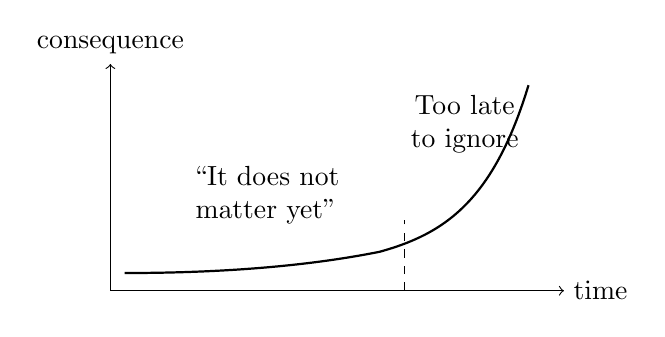
\begin{tikzpicture}[x=0.9cm,y=0.9cm]
\draw[->] (0,0) -- (6.4,0) node[right] {time};
\draw[->] (0,0) -- (0,3.2) node[above] {consequence};
\draw[thick] (0.2,0.25) .. controls (1.6,0.25) and (2.8,0.35) .. (3.8,0.55)
              .. controls (4.7,0.8) and (5.4,1.25) .. (5.9,2.9);
\draw[dashed] (4.15,0) -- (4.15,1.0);
\node[align=center] at (2.2,1.35) {``It does not\\matter yet''};
\node[align=center] at (5.0,2.35) {Too late\\to ignore};
\end{tikzpicture}
\end{adjustbox}
\end{center}

This curve is not only about markets or technology. It is also about personal concepts.

The value of writing may look flat until you need to persuade, teach, sell, raise capital, organize a team, or clarify your own thinking. The value of understanding policy may look flat until a rule changes the economics of your industry. The value of learning to invest may look flat until inflation, opportunity, or retirement forces the issue. The value of metacognition may look flat until emotion, fear, greed, or pride destroys a decision.

The curve punishes people who only learn after obvious necessity.

Wealth freedom requires earlier recognition. The person who waits until every concept is visibly relevant is late by design.

\section*{Second Chances Are Rare}

I was lucky.

Somehow, after missing that afternoon, I met the same class of ideas again through another path. I entered investing, met founders, studied markets, made mistakes, and slowly recovered concepts that may have been planted years earlier. I cannot even say clearly which ideas I learned later and which ones Zhuang Yi had already placed in front of me. Perhaps the seed was there and only took years to sprout. Perhaps I relearned everything the hard way.

It does not matter.

What matters is that six or seven years passed.

That is the chilling part. A person can miss an idea, continue living normally, and lose years without any dramatic warning. Life does not always announce, ``This is the turning point.'' Often the turning point looks like an ordinary conversation, an article, a book, a policy document, a class, a comment, or a quiet suggestion from someone who sees farther than you do.

Second chances exist, but they are not a plan.

If wealth freedom is built from attention, capital, judgment, and time, then missing an important idea is not a small matter. It is not merely ``not learning something.'' It is leaving a possible future unopened.

\section*{Bring the Idea Near}

The antidote is a habit:

\begin{quote}
Whenever an idea feels unrelated, treat that feeling as a signal to investigate, not as a conclusion.
\end{quote}

Ask:

\begin{itemize}
\item Why do I want this to be unrelated?
\item What difficulty would appear if I admitted it might apply to me?
\item Which identity am I protecting?
\item What small experiment would create contact with the idea?
\item Who already lives as if this idea is obvious?
\item What would I record if I took this seriously for seven days?
\end{itemize}

These questions do not guarantee transformation. They do something more basic: they keep the door open.

An idea becomes related by use. If you absorb it, test it, write about it, teach it, act on it, and revise your behavior around it, then it is related. If you merely agree with it, admire it, and leave it untouched, then it remains decoration.

Do the thing hard enough to create contact. Think about it deeply enough to create structure. Repeat it enough to create familiarity. Record it clearly enough to create memory.

Otherwise, the idea may have passed through your life without entering it.

\section*{The Practice}

For the next serious idea you meet, do not allow the first reaction to be distance.

Use this small practice:

\begin{enumerate}
\item Copy the idea in one sentence.
\item Write: ``At first I feel this is unrelated because \ldots''
\item Write three possible connections to your work, money, learning, relationships, or future.
\item Choose the smallest action that tests one connection.
\item Do it before the day ends.
\item Record the result, however small.
\end{enumerate}

This practice looks almost too simple. That is exactly why it is easy to miss.

Many important ideas wear the disguise of simplicity. Others wear the disguise of impossibility. The most dangerous ones wear the disguise of irrelevance.

Do not trust that disguise.

In the path toward wealth freedom, the expensive error is not only spending attention on the wrong things. It is also refusing to spend attention on the right things when they first appear, because they have not yet become obvious.

By the time they are obvious, the curve may already be steep.
